\section{Introduction}\label{sec:introduction}
Medical care providers receive insurance payment incentives to make ``meaningful use'' of electronic health records (EHRs) for tracking patient care. EHRs are an extension of electronic medical records (EMRs), the latter being simple electronic documentation of a patient's medical history. EHRs differ from EMRs in that they are meant to be shared between medical institutions and attached to a patient rather than a hospital. In theory, a single EHR could exist per patient, and any certified care provider could access any patient's up-to-date EHR. In practice, however, EHRs are fragmented among hospitals and producing EHRs is a major burden on medical care providers.

There are two explicitly stated goals of EHRs that have not been realized:
\begin{enumerate}
	\item To make medical records follow a patient seamlessly between medical institutions, and
	\item to improve quality and efficiency of medical care, by making physicians' jobs easier \cite{Meaningful-Use}.
\end{enumerate}

Why has the goal of a single, shared EHR per patient not been realized? The core problem is that each medical institution owns its own EHR system, and EHRs are not shared by default. That is, when a patient wants to move to a new institution, in most cases the new provider must explicitly request the EHR transfer. Thus the default case is that each provider maintains its own records, as it requires extra work to share the records. This contrasts with a theoretical shared-system arrangement, where the EHR is pushed to a central repository whenever it is updated.

The overhead of sharing EHRs increases when different hospitals use different EHR software. Each EHR software suite uses a proprietary internal representation of health records, which must be serialized to a standard format before sending. Fortunately, Obamacare's meaningful use regulations require that all EHR software be able to export records to an acceptable standard format. Such exported documents are called \textit{Continuity of Care Documents} (CCDs), and the regulations are outlined in \cite{CCD}. It is not always easy to generate CCDs, and the exported document is often a stripped down version of the full internal EHR. Still, as we will discuss in section~\ref{sec:obstacles}, this exportability requirement is critical for transitioning to our vision for a cloud-based sharable EHR system.

Why has the second unrealized goal -- to enable physicians to improve quality and efficiency of medical care -- not been realized? Surveys of physicians suggest that usability of EHR software plays a major role. EHR system users perennially complain that they are dissatisfied with the user experience of their software, with satisfaction levels hovering around 34\% \cite{EHR-Satisfaction}. One explanation for this shortcoming is that the purchasing structure for EHR software provides little opportunity for users to reward well designed software. A typical EHR licensing agreement goes as follows: Administrators at a large hospital enter into a contract with an EHR software company, and the physicians working in that hospital have little say in the contract. Since the dealmakers are not the users, there is no direct feedback loop to value the software based on its usability. Among EHR systems that satisfy meaningful use requirements, the hospital is likely to choose the lowest cost system, considering usability to be a secondary concern. Moreover, contracts often span multiple years, and it is difficult to move between EHR software providers.

In this paper, we suggest an alternative industry structure for electronic health record management. In our new arrangement, a single entity provides a universal cloud-based EHR database service with no frills. Companies are allowed to compete to provide tools that access the universal database, but they are required to write all changes to the monolithic service. We argue that separation of these two components -- universal cloud-based storage and a stateless EHR management tier -- offers large advantages over the current system of full-stack EHR software. In section \ref{sec:overview}, we provide an overview of our vision for cloud-based, sharable EHRs. We follow up in section \ref{sec:benefits-database} by describing the potential benefits of a single monolithic EHR database, and in section \ref{sec:benefits-stateless} we describe benefits arising from the requirement of stateless EHR management software. In section \ref{sec:obstacles}, we outline potential obstacles. We conclude in section \ref{sec:conclusion} with a summary of our vision for the EHR software industry.

\section{System overview}\label{sec:overview}
The foundation of our architecture for EHR management is a universal cloud-based EHR storage service mediated by a tier of stateless EHR software. Figure \ref{fig:system-diagram} outlines this design: Each hospital may choose to use any of the stateless EHR software products, which are offered by competing companies. Each intermediate software suite plugs into a single universal EHR database, which lives in the cloud. Since all EHR software tools access the same underlying data store, a hospital's access to any given EHR is not limited by its choice of middle-tier software.

This stands in stark contrast to today's EHR market. Currently there are many EHR software providers, each of which aims to provide a full-stack EHR management product, from storage to user interface. Moreover, these providers frequently offer systems which store records in on-premise databases, and records are owned and managed by the medical institutions themselves. In this section we describe the details of each layer our hypothetical system.

\begin{figure}
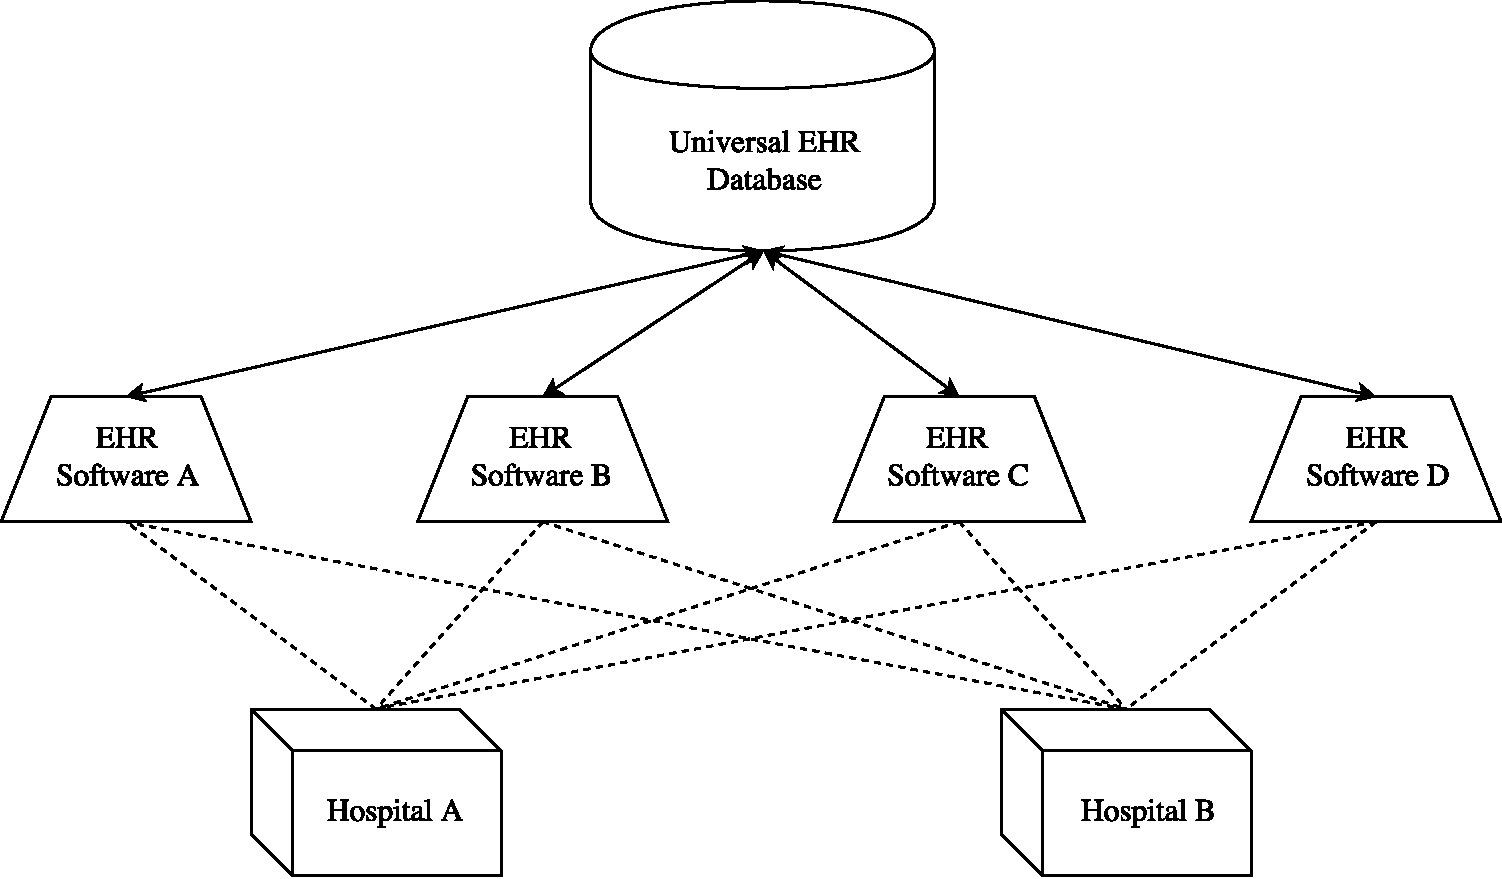
\includegraphics[scale=0.3]{system-diagram}
\caption{Universal EHR database is mediated by competing stateless EHR software products. Medical institutions choose any stateless middle-tier software and automatically have access to all EHRs.}
\label{fig:system-diagram}
\end{figure}

\subsection{Universal EHR database in the cloud}\label{sec:database}
Today's cloud providers already offer the building blocks needed to support a monolithic EHR database in the cloud. For instance, Amazon Web Services' S3 storage system provides inexpensive, massive-scale storage with built-in fault tolerance \cite{aws-s3}. While S3 is not necessarily the optimal infrastructure for a universal EHR storage system, it has proven effective for building huge, read-mostly databases (e.g., Netflix's video storage system, described in \cite{netflix-s3}). The particular cloud provider and service used for underlying infrastructure is unimportant for our purposes, thus we will just refer to this building block as the \textit{persistent cloud storage} (PCS) service.

On top of PCS, a single entity provides primitive APIs for reading and writing EHRs, as well as authentication. The database tier does not provide sophisticated features such as statistical analysis or a Web portal. A primitive database is desirable since there is no competition at the database tier: Since our design inherently relies upon a single EHR database, there is no competition to drive innovation at the storage layer. For undifferentiated primitives such as reading and writing, little innovation is necessary. However, for more advanced features that EHR software might provide, competitive pressures must be present to reward quality and usability. Therefore we push as much functionality as possible to the stateless EHR software tier.

\subsection{Stateless EHR software}\label{sec:stateless}
From the perspective of a medical care provider, all interaction with EHRs goes through a stateless EHR software product. The market for creating such products is open, so that a wide variety of competitive options for middle-tier EHR software may arise. These products must be stateless in the sense that all read operations must be pulled from, and all write operations pushed to, the database tier. Requiring statelessness ensures that medical institutions can move freely between EHR software products without losing any access to patient information.

The middle-tier software authors have free reign to implement sophisticated EHR management and analysis tools. It is likely that a number of simple portals for reading and updating EHRs would arise. Other more advanced tools would have access to the same dataset, opening the door for specialization in difficult tasks. For instance, given authenticated access to a volume of records, an EHR software suite might provide a graphical user interface to display statistics about a pool of patients. As another example, a middle-tier product might specialize in large scale analysis of EHRs. We discuss in detail the benefits of a stateless layer of EHR software in section \ref{sec:benefits-stateless}.

\section{Benefits of universal EHR storage}\label{sec:benefits-database}
Moving all EHRs to a universal cloud-based storage tier solves many problems that plague medical care providers today. First, it makes EHRs truly sharable. Experience since Obamacare's enactment has shown that the ability to share EHRs does not necessarily cause EHRs to be shared in practice. In our proposed arrangement, a universal database makes it impossible \textit{not} to share EHRs. Second, a universal EHR database forces convergence of document formats to the schema used by the monolithic storage tier. Third, a massive, well formatted pool of EHRs opens the door for unprecedented medical research opportunities.

\subsection{Automatic sharing of records}
A universal, cloud-based EHR database primarily solves the issue of sharing EHRs between care providers. To see this benefit in action, consider the situation where a patient moves to a new city and must visit a new hospital. No matter what middle-tier software was used to write the patient's EHR, the new hospital will have automatic access the patient's EHR, since it is guaranteed to reside in the universal EHR database. From the perspective of a physician, accessing the record of a new patient is equivalent to accessing the record of a returning patient. Thus sharing becomes the default mode of operation when EHR storage moves to a universal database in the cloud.

\subsection{EHR format convergence}
The migration of EHRs from previous storage systems to the universal EHR database will cause a convergence of EHR formats. EHR software providers today use a variety of proprietary storage formats. This amplifies the difficulty of switching EHR software suites, since a hospital must spend resources to convert their EHRs to the new format. Thus the ``lock in'' effect in EHR software is not just a matter of physical access, but also one of formatting. A related issue is that a proliferation of EHR formatting standards limits researchers' access to large datasets.

\subsection{Research opportunities}
For cutting edge medical research, access to large datasets is critical. Many developing techniques rely on machine learning algorithms, which derive their effectiveness from massive amounts of data. EHRs present an enticing array of features on which to train machine learning models. By moving EHRs to a universal database in the cloud, researchers gain access to an unprecedented scale of medical data in one location. Although privacy concerns must be addressed, the creation of a universal EHR database has lifesaving potential for this benefit alone.

\section{Benefits of stateless EHR software}\label{sec:benefits-stateless}
Why does our system include a stateless middle-tier of EHR software products? One could imagine an alternative design, in which the monolithic database provides a single full-featured interface, accessed directly by hospitals. The foremost issue with this arrangement is the lack of competition and, consequently, lack of pressure for innovation. A second alternative might allow the middle-tier software to maintain its own database of EHRs, only optionally pushing to the universal database. This approach would undermine the usefulness of having a monolithic database, since sharing would no longer be automatic.

In this section, we describe the benefits of the middle tier of our system. A tier of competitive, stateless EHR software offerings creates a market structure that incentivizes innovation. The ability to quickly move between middle-tier providers tightens the feedback loop for software authors. Finally, a single repository of EHRs opens the door for specialization in EHR software and introduces a clean separation of storage and presentation.

\subsection{Competitive market structure}
By making it easy to move between EHR software suites, our system eliminates any artificial forces tying hospitals to EHR software providers. In today's EHR market, it takes a non-trivial amount of work to switch between EHR systems. The transfer work can be categorized into two components: retraining and data transfer. While our system does not eliminate retraining overhead, the statelessness of EHR software ensures that no data transfer is needed. Thus care providers have a much lower cost of moving to a new EHR software system.

When it becomes cheaper to move between EHR software prov\-id\-ers, the vendors must compete more fiercely to retain customers. If one software vendor provides a more usable interface or new features, a hospital may choose to migrate to that new software system at any point. This competitive pressure drives innovation that is lacking in the market for EHR software today.

\subsection{Tighter feedback loop}
Eliminating hospital-vendor contracts tightens the feedback loop for improving EHR software. In the world of product development, iterative feedback from consumers is essential. This concept plays little role in the current EHR software market, since long-term contracts make this feedback loop take years. With stateless EHR software, a customer may switch EHR software providers in a matter of hours, rather than weeks or months. Thus EHR software authors receive much faster feedback on the quality of their tools, leading to faster innovation.

\subsection{Specialization}
By separating storage and presentation layers, we open the door for specialization in middle-tier software. First consider the current arrangement in EHR software: If a company wants to sell specialized analysis tools, for instance, it must either build a full-fledged EHR management suite, or build an analysis module that can read the storage formats of all other EHR software vendors it wishes to support. This contrasts with our proposed solution, in which an analysis tool would only need to read from the universal data tier.

This arrangement creates a proliferation of tools that focus on one task and do it well (\textit{e.g.,} predictive analytics, graphical displays, advanced search). From the software authors' perspective, focusing on specialized tools is desirable because it reduces the complexity of a system. From a care provider's perspective, modular, specialized software is also desirable. Rather than purchasing bloated, full-featured tools, hospitals can instead purchase just those specialized tools which they need. Perhaps most importantly, physicians only need to interact with those tools which they need for their jobs, instead of wading through complex dialogs.

\subsection{Separation of Concerns}
From a software engineering and systems design perspective, the two-tier design is appealing for its separation of concerns. This principle of abstraction is taught in computer science classrooms for reasons that apply here as well: Abstraction reduces duplicated logic, makes systems extensible, and helps control complexity.

First and foremost, the stateless layer avoids duplicated logic. EHR systems today must all implement their own EHR storage code (likely on top of a database engine), differing only in the on-disk format of the records. In our design, only a single EHR storage engine needs to be written and maintained. All middle-tier software benefits from performance improvements to the underlying data tier, and the cost of development is reduced. Separating the presentation logic from the database also controls the complexity of the whole system, with a clean interface on top of which all EHR software runs.

\section{Obstacles}\label{sec:obstacles}

A number of major obstacles stand in the way of our vision for EHR management systems. These hurdles range from logistical (\textit{e.g.,} importing EHRs from current databases) to legal and philosophical (\textit{e.g.,} ensuring patient privacy in a multi-tenant cloud environment). Although our treatment of these concerns is not exhaustive, we address a number of obstacles and show that, at least in theory, none are insurmountable.

\subsection{EHR migration}

To achieve the goal of a monolithic, cloud-based EHR database, there must be a phase of migration from current EHR databases. Given the large number of formats in use today, conversion to a single format is a daunting task. Thankfully, this problem is ameliorated by a clause in Obamacare's meaningful use policies. In particular, Obamacare requires EHR software to support exporting files to one of a handful of standard formats \cite{Meaningful-Use}. One such format is the Clinical Document Architecture (CDA) format, an XML-based scheme that encodes a patient's entire medical history in a text file.

Using CDA documents as a bottleneck for serialization, the migration to a universal database could work as follows. Suppose an EHR software provider wants to sell middle-tier software that accesses the universal EHR database. To gain this licensing privilege, the software vendor must update all existing offerings to allow users to upload their entire set of EHRs to the universal database. This agreement would align the interests of physicians, who will want their records in the universal database, and the EHR companies, who will want to sell middle-tier software products.

\subsection{Payment for database tier}
The PCS service must be paid for, and the database layer requires a large investment to build and maintain. Who should pay for these costs? One idea is that the entity in charge of building the database tier charges each middle-tier software provider on a pro-rated basis. The middle-tier providers could choose to pass these costs onto their customers if they wished, or they could bill using a different model and try to extract a margin from the payment structure.

Aside from the logistical concerns outlined above, there are ethical and legal questions surrounding the payment structure. Is it ethical for the universal EHR database provider to profit off of selling access to patient records? In a sense, today's EHR software providers must answer the same questions. However, the nature of pay-as-you-go billing for cloud services makes it different from the typical contract model of EHR software today. If hospitals must pay per access, then access to a patient's information is being directly sold by the database provider.

We propose two alternative payment structures that may address these concerns. First, the universal database tier could be built and managed by a nonprofit or government organization. This would ameliorate concerns that the universal database was being used for anything other than public good. Admittedly, this solution may introduce inefficiencies. Second, a for-profit entity could manage the database tier, but charge only for large-scale access to anonymized data. Since this data is highly valuable for research purposes (\textit{e.g.,} machine learning model training), it is plausible that the database provider could recover its costs in this way.

\subsection{Trust and privacy}
Medical records present challenges in that they contain highly sensitive personal information. First off, the PCS system used for storage infrastructure must be provided by a trusted company. This is a secondary concern, since large cloud providers such as Amazon and Microsoft are already trusted on a daily basis with highly sensitive information on their clouds. A more legitimate concern is that the universal EHR database tier be developed by a trustworthy company. It would be difficult for a startup company, lacking any track record of security, to build the universal database and be trusted by patients and EHR providers.

We propose that one of the large cloud providers should -- and inevitably will try to -- provide this monolithic EHR database service themselves. This would bootstrap the trust process, since these companies have already developed strong reputations for trust. Moreover, these companies have the technical knowledge of their own systems to optimize the database tier. The simple API offered by the database tier would not be much different from the APIs already provided by these companies for services such as AWS S3. Thus Amazon, Microsoft, and Google are all well positioned to provide this service in the near future.

\subsection{Regulation}
Government regulation of medical records is perhaps the most likely showstopper for our proposed EHR system. First there is the potential for U.S. anti-trust laws to eliminate the possibility of a single EHR database provider. There is another possibility that it is too difficult to satisfy HIPAA and other regulations with monolithic database in the cloud.

To address the concern of monopoly law, this system may have to come with the U.S. government's blessing. Such an arrangement does have precedent in industries where a monopoly provider has clear advantages for the public good. For instance, electrical utility companies are often granted monopolies in the United States. In a similar arrangement, it is possible that a universal EHR database provider would be granted monopoly status and have its prices regulated.

In terms of HIPAA compliance, cloud service providers already offer special services to satisfy government regulations \cite{HIPAA}. Therefore this concern is easily addressed by using a PCS service that is HIPAA-compliant.

\subsection{Resistance from current EHR companies}
The current EHR software market is lucrative, and the transition to our proposed architecture would incur significant cost to EHR software providers. As outlined above, the stateless-tier software market is designed to be highly competitive, an undesirable situation from the perspective of today's providers. As a result, dominant players are likely to resist the two-tier design proposed here.

We are hopeful that medical care providers will recognize the advantages of our system, and will provide the necessary pressure to overcome this resistance. If hospitals simply stop entering contracts for traditional EHR software, then existing companies will be forced to provide stateless EHR solutions or risk going bankrupt.

\section{Conclusions}\label{sec:conclusion}
In this paper, we have presented a new architecture for EHR management in the cloud. The new system is composed of two distinct tiers: A monolithic database layer that stores all EHRs in the cloud, and a layer of stateless EHR software products that must maintain consistency with the universal database. Such a design has many advantages over today's EHR solutions. Most importantly, our system makes it automatic to share records between medical institutions. It eliminates data lock-in for hospitals, thereby creating a more competitive market for EHR software systems and incentivizing software vendors to design more usable products.

To implement our system, we suggest that two major forces must come together. First, an established, trustworthy entity (\textit{e.g.,} a major cloud provider) must offer a universal EHR database service on top of persistent cloud storage. Second, government policies must facilitate this arrangement, perhaps by granting monopoly privileges to the universal database provider. If these two forces come together, the overwhelming advantages of our system's architecture will make today's EHR systems obsolete. When that day arrives, medical care providers will finally have access to the sharable, usable EHRs that have long been the holy grail of healthcare IT.

%\begin{acks}
%
%\end{acks}






























